\documentclass[manuscript,review]{acmart}
\usepackage{graphicx} % Required for inserting images
\usepackage{hyperref}
\usepackage{amsmath}
\usepackage{amssymb}
\usepackage{booktabs}
\usepackage{wrapfig}
\usepackage{algorithm}
\usepackage{algorithmic}

\title{Joint Relational Database Generation via Graph-Conditional Diffusion Models}

\begin{document}

\author{Mohamed Amine Ketata}
\email{a.ketata@tum.de}
\affiliation{
    \institution{School of Computation, Information and Technology \& Munich Data Science Institute, Technical University of Munich}
    \country{Germany}
}

\author{David Lüdke}\
\affiliation{
    \institution{School of Computation, Information and Technology \& Munich Data Science Institute, Technical University of Munich}
    \country{Germany}
}

\author{Leo Schwinn}
\affiliation{
    \institution{School of Computation, Information and Technology \& Munich Data Science Institute, Technical University of Munich}
    \country{Germany}
}

\author{Stephan Günnemann}
\affiliation{
    \institution{School of Computation, Information and Technology \& Munich Data Science Institute, Technical University of Munich}
    \country{Germany}
}

\begin{abstract}
    Building generative models for relational databases (RDBs) is important for many applications, such as privacy-preserving data release and augmenting real datasets. However, most prior works either focus on single-table generation or adapt single table models to the multi-table setting by relying on autoregressive factorizations and sequential generation. These approaches limit parallelism, restrict flexibility in downstream applications, and compound errors due to commonly made conditional independence assumptions. In this paper, we propose a fundamentally different approach: jointly modeling all tables in an RDB without imposing any table order. By using a natural graph representation of RDBs, we propose the Graph-Conditional Relational Diffusion Model (GRDM), which leverages a graph neural network to jointly denoise row attributes and capture complex inter-table dependencies. Extensive experiments on six real-world RDBs demonstrate that our approach substantially outperforms autoregressive baselines in modeling multi-hop inter-table correlations and achieves state-of-the-art performance on single-table fidelity metrics. Our code is available at \url{https://github.com/ketatam/rdb-diffusion.}
\end{abstract}

\maketitle

\section{Introduction}
Relational databases (RDBs) are essential for modern data management. They hold around 70\% of the worlds data\cite{dbengines2023} across key sectors like healthcare, finance and e-commerce\cite{PhysioNet-mimiciii-1.4}. However, using this vast amount of data is increasingly hindered by strict privacy laws. While these regulations are crucial for safe-guarding sensitive personal information, they create obstacles for researchers who need rich data to create useful data-driven technologies.

To close the gap between data privacy and data usefulness, synthetic data generation\cite{RUJAS2025105763} has become an important solution. By training generative AI models on private, real world databases, we can create completely synthetic databases. These synthetic datasets maintain the complex statistical structure and pattern of the original data but do not include any sensitive records, making them safe to share and analyze.

Although there has been progress in generating synthetic data for single tables, creating complex multi-table relational databases is still a challenging and less explored issue. The main drawback of current multi-table generation methods is their dependence on autoregressive frameworks. These traditional approaches require the models to generate tables in a strict order. This sequential process limit the model's flexibility for later tasks, like filling in missing data, prevents parallel data generation, and makes it hard for the model to capture deep, long range connections across multiple linked tables. Additionally, these older methods often make simplifying assumptions about conditional independence which lowers the overall quality and accuracy of generated data.

To tackle the significant challenges of sequential generation, this paper presents a completely new approach: a joint modeling method that removes the need for a set table order. The authors propose the first non-autoregressive generative model designed specifically for relational databases.
\begin{wrapfigure}{r}
    \centering
    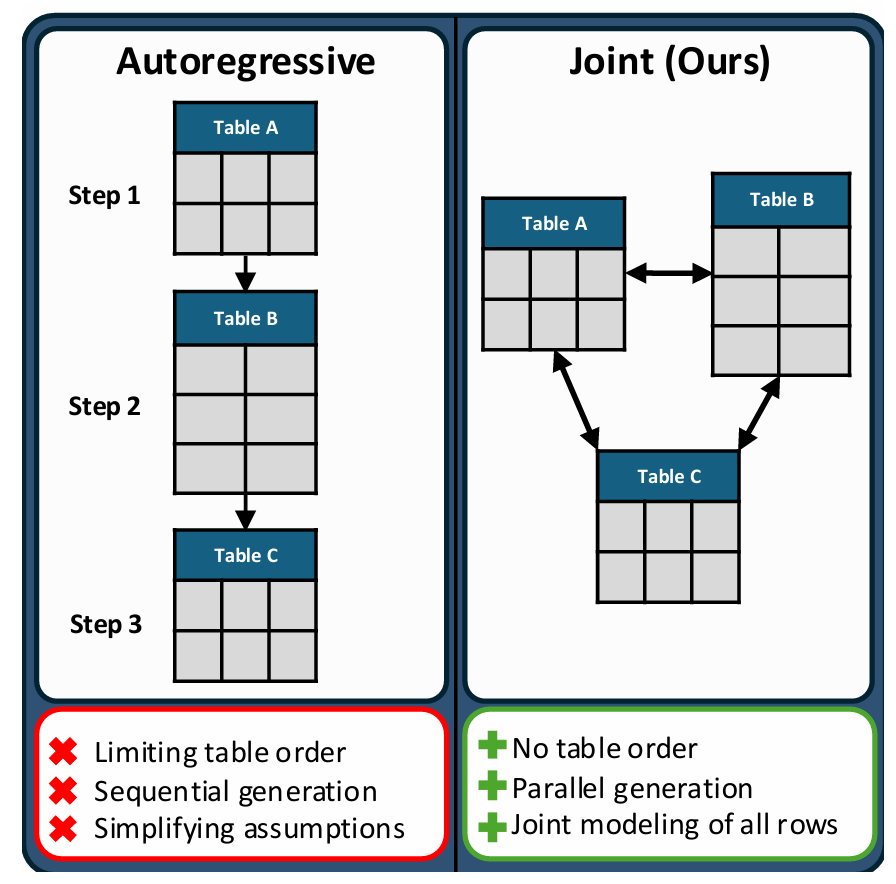
\includegraphics[width=0.5\linewidth]{figures/figure1.png}
    \caption{Figure 1: Comparison of autoregressive and joint relational database generation.}
    \label{fig:1}
\end{wrapfigure}
The main innovation of this approach is the view of a relational database as a flexible graph rather than a strict hierarchy of tables. In this graph, individual rows of data act as "nodes," while the primary-foreign key relationships connecting them serve as "edges." By framing database generation as a graph generation task, the authors introduce the Graph-Conditional Relational Diffusion Model (GRDM). This model works in two separate phases: first, it samples a realistic graph structure that resembles the original database's connections, and then it uses a graph neural network combined with a diffusion process to generate the actual data attributes for all rows at the same time.

The authors highlight three main contributions in this study:
\begin{itemize}
    \item The introduction of a new generative framework that models the joint distribution of all tables in a database at once, moving away from the limiting autoregressive methods used in previous research.
    \item The development of GRDM, a groundbreaking non-autoregressive model that uses graph representations to jointly clean and generate row attributes throughout the entire database.
    \item Strong empirical evidence showing that GRDM significantly outperforms existing autoregressive methods across six different, real-world relational databases, demonstrating an exceptional ability to capture complex, inter-table dependencies.
\end{itemize}

\section{Background}
\textbf{Relational Databases.} A Relational Database (RDB) organizes information into a set of interconnected tables, guided by a predefined schema that dictates how these tables relate to one another. Each row within a table represents a unique entity instance and is constructed from three main components: a primary key (a unique identifier for the row), foreign keys (references pointing to primary keys in parent tables), and attributes (the actual data features, which can be numerical, categorical, or temporal). 

The primary objective of synthetic RDB generation is to learn the underlying data distribution of the original database so that a new, artificial database can be sampled. This synthetic version must adhere to the original structural schema while accurately preserving the statistical properties of the real data. This is a highly challenging task because the model must learn both the complex, multi-modal distributions of individual columns and the intricate correlations that exist not only within a single table but across multiple tables connected via primary-foreign key links.

As a natural way to represent this structure, an RDB can be viewed as a graph, where each row is a node and each primary-foreign key link is an edge. Figure\ref{fig:2} illustrates this correspondence between the tabular and graph views.
\begin{figure}[t]
    \centering
    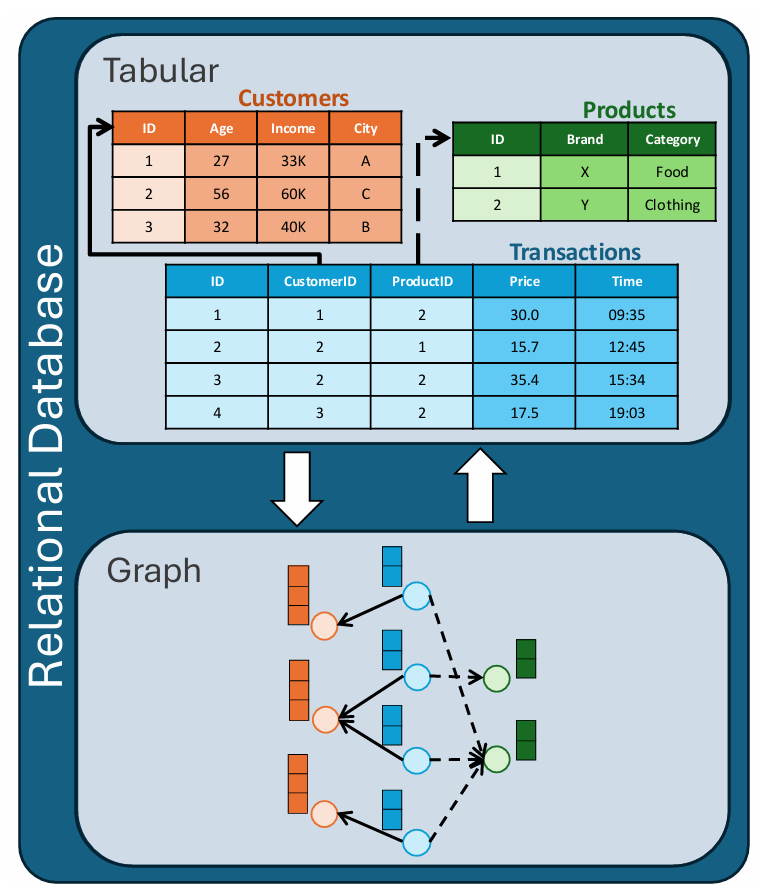
\includegraphics[width=0.4\linewidth]{figures/figure2.png}
    \caption{Tabular and graph representations of relational databases.}
    \label{fig:2}
\end{figure}
With this graph representation $G = (V, E, X)$, where $V$ is the set of nodes, $E$ is the set of edges, and $X$ the node features, the target data distribution becomes:
\begin{equation}
    p_\theta(R) = p_\theta(V,E,X)
    \label{eq:target}
\end{equation}
\subsection{Limitations of Autoregressive Models}
Historically, generative models for relational databases have relied on autoregressive factorization. This means they impose a strict topological order on the tables and generate them sequentially—one after another, conditioned on the tables that were generated previously. 

While these models can theoretically model joint distributions, this sequential nature leads to significant practical issues. First, a fixed table order limits how useful the synthetic data is in later tasks, such as filling in missing values because a table cannot easily get context from tables that come later in the generation sequence. Second, the sequential process cannot be easily parallelized, making it slow and expensive for large databases. Finally, to simplify the sequential learning process, earlier methods often made conditional independence assumptions. In an autoregressive setting, these assumptions present problems because small errors during generation add up at each step, quickly reducing the coherence and accuracy of the resulting data.

\subsection{Related Work}
The field of synthetic data generation has advanced quickly. For single-table data, early methods relied on Bayesian networks and Generative Adversarial Networks (GANs) such as CTGAN~\cite{NEURIPS2019_254ed7d2}, while more recent diffusion-based approaches like TabDDPM~\cite{pmlr-v202-kotelnikov23a} and TabSyn~\cite{zhang2024mixedtypetabulardatasynthesis} achieve stronger performance on complex tabular distributions.

For multi-table relational databases, foundational work such as the Synthetic Data Vault (SDV)~\cite{7796926} used Gaussian copula models, and more recent methods like ClavaDDPM~\cite{NEURIPS2024_98387657} adapt diffusion models to relational data. Regardless of the underlying model class, these approaches all share the same limitation: they rely on autoregressive, sequential generation.

Our approach also draws on the broader graph generation literature. Social and citation network models typically involve complex structures with simple node features, whereas RDB-derived graphs exhibit the opposite: simple, highly structured topologies with complex, multi-modal node attributes. This combination of graph structure and tabular complexity is the central challenge our joint modeling framework addresses.

\section{Method}
We introduce a non-autoregressive generative model for relational databases by modeling the joint distribution over all tables directly, rather than factorizing it sequentially. This section first describes how we represent an RDB as a graph (Section \ref{sec:graph-rep}), then explains our two-step generation procedure: sampling the graph structure, followed by generating node features with our diffusion model.

\subsection{Relational Databases as Graphs}
\label{sec:graph-rep}
We represent an RDB as a directed, heterogeneous graph $G = (V, E, X)$. Each row in the database becomes a node, with node types corresponding to table types. Primary-foreign key references between rows become directed edges, typed by the tables they connect. The non-key attributes of each row form that node's feature vector, collected in $X$. Because edges alone encode the primary and foreign keys, this representation fully preserves the relational structure of the original database and can be converted back into tables.

\subsection{Factorizing the Joint Distribution}
To find a scalable way to model $p_\theta(V,E,X)$ we consider three possible factorizations: generating everything at once, generating features and then edges, or generating edges and then features:
\begin{align}
    \text{(A) One-shot:} \quad & p(V,E,X) \\
    \text{(B) Features-then-edges:} \quad & p(V,X)\, p(E \mid V, X) \\
     \text{(C) Edges-then-features:} \quad & p(V, E)\, p(X \mid V, E) \\
\end{align}
Factorizations (A) and (B) require considering every possible pair of nodes as a candidate edge, which becomes computationally infeasible as the database grows. Factorization (C) avoids this by generating the graph structure first, allowing the number of edges and their types to be sampled efficiently before any node features are considered. We therefore adopt factorization (C):
\begin{equation}
    p(V,E,X) = p(V,E)\, p(X \mid V,E)
    \label{eq:factorization}
\end{equation}
This corresponds to a two step process: first sampling the graph structure $p(V,E)$ (Section~\ref{sec:graph-rep}), then generating node features $p(X \mid V,E)$ using our diffusion model (Section~\ref{sec:grdm}).

\subsection{Node Degree Preserving Random Graph Generation}
\label{sec:graph-gen}
To model $p(V, E)$, we use a random graph generation procedure that preserves the indegree distribution of each edge type as observed in the real database. Outdegrees are fixed by the schema, since each table has a set number of foreign key columns, so only indegrees need to be modeled. Generation starts from root nodes (rows with no outgoing foreign keys) and recursively samples child nodes according to the learned indegree distributions. When a node ends up with multiple parents, duplicate copies created during this process are merged via random matching, preserving the overall degree distribution while producing a valid graph.

\subsection{Graph-Conditional Relational Diffusion Model (GRDM)}
\label{sec:grdm}
Given a fixed graph structure $(V,E)$, we now generate the node features $X$. This This is analogous to image generation, where an image is a graph with a regular grid structure and each pixel is a node with a color feature vector. Here, we generate a much larger and more irregular "image" defined by the database's graph structure. Motivated by the success of diffusion models in image generation, we model $p(X \mid V, E)$ using a diffusion process, treating it as a generalization of image diffusion to graphs with arbitrary structure and heterogeneous node features. We denote the original node features as $X^{(0)}$, following standard diffusion model notation.

\subsection{Forward Process}
Diffusion models Diffusion models define a fixed Markov chain, the \emph{forward process}, that gradually adds noise to the data across $T$ timesteps, producing a sequence of increasingly noisy latents $X^{(1)}, \dots, X^{(T)}$ of the same dimensionality as $X^{(0)}$:
\begin{equation}
    q\big(X^{(1:T)} \mid X^{(0)}\big) = \prod_{t=1}^{T} q\big(X^{(t)} \mid X^{(t-1)}\big)
    \label{eq:forward-chain}
\end{equation}
We add noise independently to each node's features at every timestep, mirroringchow pixels are noised independently in image diffusion. For a given node $v$ with features $\mathbf{x}_v$, this gives:
\begin{equation}
    q\big(\mathbf{x}_v^{(t)} \mid \mathbf{x}_v^{(t-1)}\big) = \mathcal{N}\!\big(\mathbf{x}_v^{(t)};\, \sqrt{1-\beta_t}\, \mathbf{x}_v^{(t-1)},\, \beta_t \mathbf{I}\big)
    \label{eq:forward-node}
\end{equation}
where $\beta_t \in (0,1)$ is a fixed noise schedule controlling how much noise is added at step $t$.

\subsection{Reverse Process and Training}
The reverse process learns to undo the noise step by step, turning pure static back into realistic node features. We parameterize this reverse process with a graph neural network $f_\theta$ that makes the noisy graph at step $t$ and predicts a denoised version:
\begin{equation}
    p_\theta\big(X^{(t-1)} \mid X^{(t)}, V, E\big) = \mathcal{N}\!\big(X^{(t-1)};\, \mu_\theta(X^{(t)}, t, V, E), \, \sigma_t^2 \mathbf{I}\big)
    \label{eq:reverse}
\end{equation}
The network is trained by minimizing the difference between the true noise added during the forward process and the noise predicted by $f_\theta$, using a simplified denoising loss:
\begin{equation}
    \mathcal{L}(\theta) = \mathbb{E}_{t, X^{(0)}, \epsilon} \Big[ \big| \epsilon - f_\theta(X^{(t)}, t, V, E) \big|^2\Big]
    \label{eq:loss}
\end{equation}
where $\epsilon$ is the random noise sampled at step $t$, and $X^{(t)}$ is obtained by applying the forward process to $X^{(0)}$. Because $f_\theta$ is a graph neural network, it naturally aggregates information from each node's neighbors, allowing the model to capture dependencies across connected rows — even across multiple hops — as denoising steps accumulate.

\subsection{Handling Dimension Tables}
Some tables in an RDB have few rows, with each row representing a unique real-world entity. For example, a table listing countries. These are known as \emph{dimension tables}~\cite{fey2023relationaldeeplearninggraph} in the RDB literature, as opposed to \emph{fact tables}, which store interactions between entities (e.g., transactions) and therefore form the bulk of an RDB's rows.
Dimension tables present a problem for generative modeling since there is no inherent concept of "generalizing" to new synthetic rows because each row is a distinct real-world entity. Therefore, instead of creating dimension tables, we treat them as fixed metadata that the rest of the model depends on. In actuality, this means that during training or sampling, we do not introduce noise to dimension table rows; instead, they remain fixed at $t=0$ throughout the diffusion process, and associations between them (such as a customer's country of residence) are nevertheless formed stochastically via the graph edges. Tables with at least one categorical column with unique values are what we refer to as dimension tables.

\subsection{Training and Sampling Procedure}
\begin{algorithm}
    \caption{Training}
    \label{alg:training}
    \begin{algorithmic}[1]
        \REPEAT
        \STATE Sample $v \sim \text{Uniform}(V)$
        \STATE $(V_{v,K}, E_{v,K}, X_{v,K}^{(0)}) \leftarrow SELECT_K(v;V,E,X^{(0)})$ \COMMENT{$K$-hop neighborhood around $v$}
        \STATE Sample $t \sim \text{Uniform}(\{1,\dots,T\})$
        \STATE Sample $\{\epsilon_{v'} \sim \mathcal{N}(\mathbf{0}, \mathbf{I}) \mid v' \in V_{v,K}\}$
        \STATE $X_{v,K}^{(t)} \leftarrow \{\sqrt{\bar\alpha_t}x_{v'}^{(0)} + \sqrt{1-\bar\alpha_t}\epsilon_{v'} \mid v' \in V_{v,K} \}$
        \STATE $\hat\epsilon_v \leftarrow \epsilon_\theta\big((V_{v,K},\epsilon_{v,K},X_{v,K}^{(t)}),t\big)$
        \STATE Take a gradient descent step on $\nabla_{theta} \|\epsilon_v - \hat\epsilon_v\|^2$
        \UNTIL{converged}
    \end{algorithmic}
\end{algorithm}



\section{Findings and Results}
\subsection{Experimental Setup}
We evaluate GRDM on six real world relational databases: Berka, Instacart 05, Movie Lens, CCS, California, and RelBench-F1~\cite{wang20244dbinfer4dbenchmarkingtoolbox} These databases vary widely in size, table count, and the complexity of their
inter-table connections, with Berka, Instacart 05, and RelBench-F1 exhibiting the most complex dependencies, including relationships spanning up to three hops. We compare against four baselines: SDV~\cite{7796926}, a statistical Gaussian-copula method; ClavaDDPM~\cite{NEURIPS2024_98387657}, a state-of-the-art autoregressive diffusion baseline; and SingleTable and Denorm, two additional pipelines that generate tables independently or after joining them, respectively. All diffusion-based methods share the same underlying architecture for a fair comparison. Fidelity is measured using four metrics: Cardinality, Column Shapes, Intra-Table Trends, and Inter-Table Trends (at increasing hop distances), all normalized to a 0--100 scale.
\subsection{Result}
GRDM consistently outperforms all baselines on Inter-Table Trends across every database, with the largest gains on databases with the most complex schemas. On Berka, GRDM improves over the best baseline by 14.14\% on 3-hop correlations and 11.3\% on 2-hop correlations. On Instacart 05, it improves 2-hop correlations by over 5.7 times, and on RelBench-F1 by 12.62\%. Averaged across all databases, GRDM achieves an 8.15\% gain on 1-hop correlations compared to the strongest baseline. These results confirm that jointly modeling all rows through the diffusion process captures long-range, multi-hop dependencies far better than autoregressive approaches. On single-table metrics (Cardinality, Column Shapes, Intra-Table Trends), GRDM performs comparably to the best baselines, and even surpasses them on some databases, despite not being specialized for single-table fidelity.
\begin{table}[t]
    \centering
    \caption{Fidelity metrics on the Berka database (most complex schema). SDV does not support databases with more than 5 tables. Improvement is GRDM vs.\ the best baseline.}
    \label{tab:berka}
    \begin{tabular}{lccccc}
         \toprule
         Metric & SDV & SingleTable & Denorm & ClavaDDPM & GRDM (Ours) \\
         \midrule
        Cardinality            &--& $97.06 \pm 0.80 $ & $96.06 \pm 1.15$ & $96.75 \pm 0.26$ & $\mathbf{99.65 \pm 0.05}$ \\
        Column Shapes          & -- & $94.58 \pm 0.01$ & $83.28 \pm 0.97$ & $94.60 \pm 0.41$ & $\mathbf{96.84 \pm 0.14}$ \\
        Intra-Table Trends      & -- & $91.72 \pm 0.23$ & $72.12 \pm 0.73$ & $90.53 \pm 1.93$ & $\mathbf{98.23 \pm 0.03}$ \\
        Inter-Table (1-hop)     & -- & $81.77 \pm 1.19$ & $55.77 \pm 2.80$ & $83.79 \pm 4.21$ & $\mathbf{91.41 \pm 0.11}$ \\
        Inter-Table (2-hop)     & -- & $78.09 \pm 0.53$ & $57.68 \pm 1.67$ & $85.87 \pm 2.72$ & $\mathbf{95.57 \pm 0.04}$ \\
        Inter-Table (3-hop)     & -- & $75.56 \pm 0.34$ & $55.59 \pm 1.48$ & $80.98 \pm 3.12$ & $\mathbf{92.43 \pm 0.69}$ \\
        \bottomrule
    \end{tabular}
\end{table}
\section{Discussion}
The current work introduces GRDM, which is the first non-autoregressive generative model designed for relational databases. Since the generation of the graph-based representation of an RDB occurs through two phases (structure first, followed by diffusion of nodes), GRDM can overcome the limitations imposed by the pre-existing models due to their reliance on the order of the tables. In this way, since each node's denoising process relies on its neighborhood (which increases as the number of diffusions increases), long-range dependencies can be captured through the use of multiple hops, which is reflected in its superior performance compared to the autoregressive baselines on six real-world RDBs.
\textbf{Limitations and Future Work.} Directions for improvement include the following. The graph generation technique, although very useful, is fairly simple in nature, and other techniques can be adopted in future for improved results. Graph representation is another modeling choice; some tables like transactions or review tables can perhaps be better represented as edge attributes rather than nodes. Furthermore, this research does not consider generation for conditional tasks; adapting GRDM to perform conditional tasks will increase its scope of utility. Finally, the authors suggest that making GRDM differentially private is necessary before adopting it in privacy-sensitive domains.

\bibliographystyle{ACM-Reference-Format}
\bibliography{references}
\end{document}
